% Created by tikzDevice version 0.10.1 on 2017-10-23 14:30:38
% !TEX encoding = UTF-8 Unicode
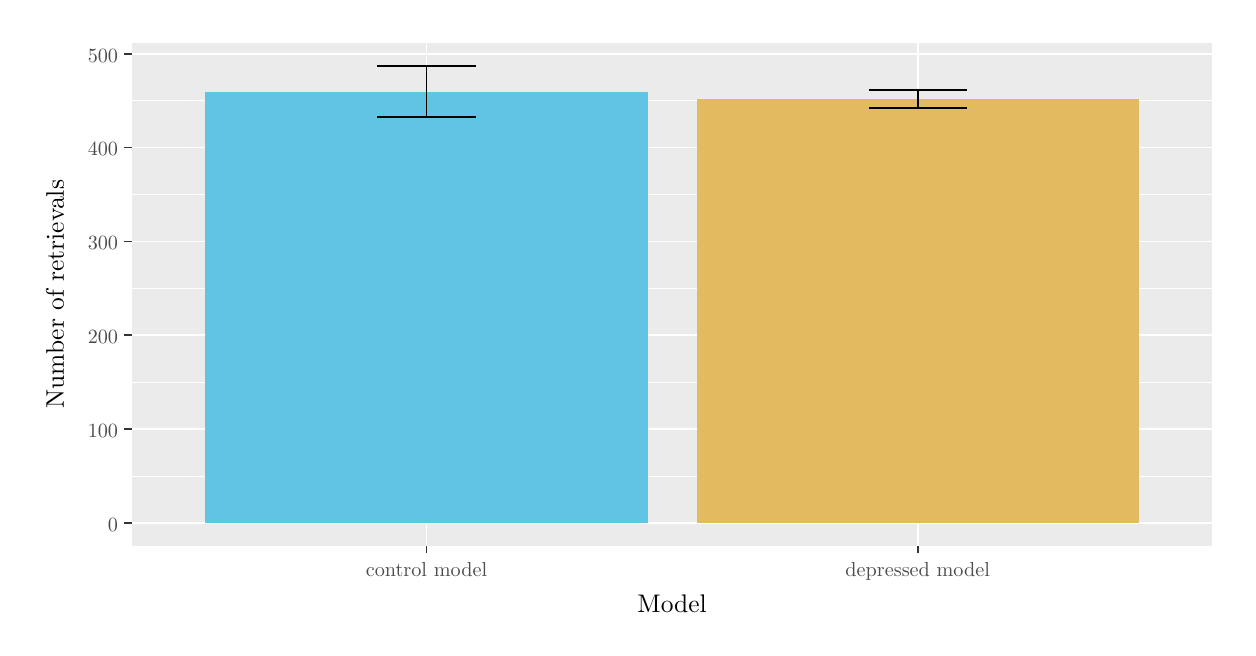
\begin{tikzpicture}[x=1pt,y=1pt]
\definecolor{fillColor}{RGB}{255,255,255}
\path[use as bounding box,fill=fillColor,fill opacity=0.00] (0,0) rectangle (433.62,216.81);
\begin{scope}
\path[clip] (  0.00,  0.00) rectangle (433.62,216.81);
\definecolor{drawColor}{RGB}{255,255,255}
\definecolor{fillColor}{RGB}{255,255,255}

\path[draw=drawColor,line width= 0.6pt,line join=round,line cap=round,fill=fillColor] (  0.00,  0.00) rectangle (433.62,216.81);
\end{scope}
\begin{scope}
\path[clip] ( 37.61, 29.59) rectangle (428.12,211.31);
\definecolor{fillColor}{gray}{0.92}

\path[fill=fillColor] ( 37.61, 29.59) rectangle (428.12,211.31);
\definecolor{drawColor}{RGB}{255,255,255}

\path[draw=drawColor,line width= 0.3pt,line join=round] ( 37.61, 54.80) --
	(428.12, 54.80);

\path[draw=drawColor,line width= 0.3pt,line join=round] ( 37.61, 88.72) --
	(428.12, 88.72);

\path[draw=drawColor,line width= 0.3pt,line join=round] ( 37.61,122.63) --
	(428.12,122.63);

\path[draw=drawColor,line width= 0.3pt,line join=round] ( 37.61,156.54) --
	(428.12,156.54);

\path[draw=drawColor,line width= 0.3pt,line join=round] ( 37.61,190.46) --
	(428.12,190.46);

\path[draw=drawColor,line width= 0.6pt,line join=round] ( 37.61, 37.85) --
	(428.12, 37.85);

\path[draw=drawColor,line width= 0.6pt,line join=round] ( 37.61, 71.76) --
	(428.12, 71.76);

\path[draw=drawColor,line width= 0.6pt,line join=round] ( 37.61,105.67) --
	(428.12,105.67);

\path[draw=drawColor,line width= 0.6pt,line join=round] ( 37.61,139.59) --
	(428.12,139.59);

\path[draw=drawColor,line width= 0.6pt,line join=round] ( 37.61,173.50) --
	(428.12,173.50);

\path[draw=drawColor,line width= 0.6pt,line join=round] ( 37.61,207.41) --
	(428.12,207.41);

\path[draw=drawColor,line width= 0.6pt,line join=round] (144.12, 29.59) --
	(144.12,211.31);

\path[draw=drawColor,line width= 0.6pt,line join=round] (321.62, 29.59) --
	(321.62,211.31);
\definecolor{fillColor}{RGB}{95,197,226}

\path[fill=fillColor] ( 64.24, 37.85) rectangle (223.99,193.74);
\definecolor{fillColor}{RGB}{226,186,95}

\path[fill=fillColor] (241.74, 37.85) rectangle (401.49,191.02);
\definecolor{drawColor}{RGB}{0,0,0}

\path[draw=drawColor,line width= 0.6pt,line join=round] (126.37,203.05) --
	(161.87,203.05);

\path[draw=drawColor,line width= 0.6pt,line join=round] (144.12,203.05) --
	(144.12,184.42);

\path[draw=drawColor,line width= 0.6pt,line join=round] (126.37,184.42) --
	(161.87,184.42);

\path[draw=drawColor,line width= 0.6pt,line join=round] (303.87,194.23) --
	(339.37,194.23);

\path[draw=drawColor,line width= 0.6pt,line join=round] (321.62,194.23) --
	(321.62,187.82);

\path[draw=drawColor,line width= 0.6pt,line join=round] (303.87,187.82) --
	(339.37,187.82);
\end{scope}
\begin{scope}
\path[clip] (  0.00,  0.00) rectangle (433.62,216.81);
\definecolor{drawColor}{gray}{0.30}

\node[text=drawColor,anchor=base east,inner sep=0pt, outer sep=0pt, scale=  0.73] at ( 32.66, 34.82) {0};

\node[text=drawColor,anchor=base east,inner sep=0pt, outer sep=0pt, scale=  0.73] at ( 32.66, 68.73) {100};

\node[text=drawColor,anchor=base east,inner sep=0pt, outer sep=0pt, scale=  0.73] at ( 32.66,102.64) {200};

\node[text=drawColor,anchor=base east,inner sep=0pt, outer sep=0pt, scale=  0.73] at ( 32.66,136.56) {300};

\node[text=drawColor,anchor=base east,inner sep=0pt, outer sep=0pt, scale=  0.73] at ( 32.66,170.47) {400};

\node[text=drawColor,anchor=base east,inner sep=0pt, outer sep=0pt, scale=  0.73] at ( 32.66,204.38) {500};
\end{scope}
\begin{scope}
\path[clip] (  0.00,  0.00) rectangle (433.62,216.81);
\definecolor{drawColor}{gray}{0.20}

\path[draw=drawColor,line width= 0.6pt,line join=round] ( 34.86, 37.85) --
	( 37.61, 37.85);

\path[draw=drawColor,line width= 0.6pt,line join=round] ( 34.86, 71.76) --
	( 37.61, 71.76);

\path[draw=drawColor,line width= 0.6pt,line join=round] ( 34.86,105.67) --
	( 37.61,105.67);

\path[draw=drawColor,line width= 0.6pt,line join=round] ( 34.86,139.59) --
	( 37.61,139.59);

\path[draw=drawColor,line width= 0.6pt,line join=round] ( 34.86,173.50) --
	( 37.61,173.50);

\path[draw=drawColor,line width= 0.6pt,line join=round] ( 34.86,207.41) --
	( 37.61,207.41);
\end{scope}
\begin{scope}
\path[clip] (  0.00,  0.00) rectangle (433.62,216.81);
\definecolor{drawColor}{gray}{0.20}

\path[draw=drawColor,line width= 0.6pt,line join=round] (144.12, 26.84) --
	(144.12, 29.59);

\path[draw=drawColor,line width= 0.6pt,line join=round] (321.62, 26.84) --
	(321.62, 29.59);
\end{scope}
\begin{scope}
\path[clip] (  0.00,  0.00) rectangle (433.62,216.81);
\definecolor{drawColor}{gray}{0.30}

\node[text=drawColor,anchor=base,inner sep=0pt, outer sep=0pt, scale=  0.73] at (144.12, 18.58) {control model};

\node[text=drawColor,anchor=base,inner sep=0pt, outer sep=0pt, scale=  0.73] at (321.62, 18.58) {depressed model};
\end{scope}
\begin{scope}
\path[clip] (  0.00,  0.00) rectangle (433.62,216.81);
\definecolor{drawColor}{RGB}{0,0,0}

\node[text=drawColor,anchor=base,inner sep=0pt, outer sep=0pt, scale=  0.92] at (232.87,  5.50) {Model};
\end{scope}
\begin{scope}
\path[clip] (  0.00,  0.00) rectangle (433.62,216.81);
\definecolor{drawColor}{RGB}{0,0,0}

\node[text=drawColor,rotate= 90.00,anchor=base,inner sep=0pt, outer sep=0pt, scale=  0.92] at ( 13.08,120.45) {Number of retrievals};
\end{scope}
\end{tikzpicture}
